\documentclass[11pt,a4paper]{article}
\usepackage{fontspec}
\setmainfont{TeX Gyre Pagella}
\newfontfamily\headfont{Inter}[UprightFont=*-ExtraBold,BoldFont=*-ExtraBold,Extension=.otf,Path=/usr/share/fonts/opentype/inter/]
\usepackage[a4paper,margin=2.3cm]{geometry}
\usepackage{graphicx,booktabs,float,caption,array,xcolor}
\usepackage[hidelinks]{hyperref}
\usepackage{titlesec}
\usepackage[round]{natbib}
\usepackage{setspace}
\setstretch{1.05}
\renewcommand{\topfraction}{0.9}
\renewcommand{\bottomfraction}{0.8}
\renewcommand{\textfraction}{0.1}
\renewcommand{\floatpagefraction}{0.75}
\setlength{\parindent}{0pt}
\setlength{\parskip}{0.55em}
\titleformat{\section}{\headfont\Large}{\thesection}{0.8em}{}
\titleformat{\subsection}{\headfont\large}{\thesubsection}{0.8em}{}
\captionsetup{font=small,labelfont=bf}
\urlstyle{same}
\hypersetup{pdftitle={The Plague Years: Five Centuries of Plague Outbreaks in Europe and the Mediterranean, 1347 to 1900},pdfauthor={Tristan Hotham}}

\begin{document}
\begin{center}
{\Large\bfseries The Plague Years\par}
\vspace{0.4em}
{\large Five centuries of plague outbreaks in Europe and the Mediterranean, 1347 to 1900,\\from a digitised copy of Biraben's inventory\par}
\vspace{1.2em}
{\large Tristan Hotham\par}
\vspace{0.3em}
{\small Independent researcher\\
ORCID: 0000-0003-4931-9349\\
DOI: \href{https://doi.org/10.5281/zenodo.23844513}{https://doi.org/10.5281/zenodo.23844513}\par}
\vspace{0.8em}
2026
\end{center}

\begin{quote}
\small
\begin{center}\textbf{Abstract}\end{center}
Plague reached the Mediterranean in 1347 and returned to European towns for more than three centuries. I describe that history using the digitisation by \citet{buntgen2012} of the inventory of plague outbreaks compiled by \citet{biraben1975}. After repairing faults in the published file (swapped latitude and longitude, a broken row, a missing-value code, repeated rows and five mislocated towns), the data hold 6,848 town-years with plague recorded in 1,172 towns, from 1347 to 1900. The first wave reached 195 towns between 1347 and 1353; a line fitted through distance and first year gives a spread of 176 to 214 km a year as the crow flies, an average over fast sea passages and slower overland spread that annual dates cannot resolve further. Outbreaks peak in the 1630s (570 town-years). The median gap between successive plague episodes in a town is 13 years (interquartile range 6 to 31). Measured by the last year with plague in three or more towns, plague left Italy (1657) and Britain and Ireland (1667) first and France by 1722, but persisted in North Africa to 1821 and in Anatolia, the Levant and Egypt to 1834. The inventory is a record of surviving documents: France alone holds 40\% of all records, eastern Europe is thin and Moscow and Constantinople are absent. The results describe the record of plague, not its full extent or its mortality.

\textbf{Keywords:} plague; Black Death; second pandemic; historical epidemiology; Biraben; digitised data; mapping; Europe; Mediterranean
\end{quote}

\section{Introduction}
The Black Death arrived in Sicily in the autumn of 1347, on ships from the Black Sea, and within five years had crossed most of Europe and the Mediterranean world, killing a large share of the population \citep{benedictow2004}. It was the start of what is now called the second plague pandemic. For more than three hundred years afterwards plague kept returning to European towns, and it did not disappear from the southern and eastern shores of the Mediterranean until the nineteenth century.

The most complete inventory of that history is the list of plague outbreaks by place and year compiled by the French demographer and historian Jean-No\"el Biraben \citep{biraben1975}. \citet{buntgen2012} digitised it, geocoded its places and published it as an open dataset \citep{envidat}, and it has since been used to study the climatic drivers of plague reintroductions \citep{schmid2015} and the network structure of its spread \citep{gomez2017}. It has also been criticised as a source that can mislead when used without regard to how it was compiled \citep{roosen2018}.

This paper does something simpler and more descriptive. It maps the digitised inventory year by year, with an interactive companion (\url{https://maps.tristanhotham.com/plague-map/}), and reports five things it shows: the spread of the first wave; the rise and fall of outbreaks over five centuries; the towns with most recorded outbreaks; how often plague returned to a town; and when it last appeared in each region and country. Throughout, I try to separate what the record says about plague from what it says about records.

\section{Data}
\subsection{The digitised inventory}
\citet{buntgen2012} published a table of 6,929 rows, each a place, a year of outbreak and coordinates in two systems: ETRS89 Lambert azimuthal equal-area (EPSG:3035) and WGS84 latitude and longitude. The dataset is held on EnviDat \citep{envidat} under the Open Database Licence (ODbL) 1.0, with the Database Contents Licence. The underlying inventory is Biraben's \citep{biraben1975}, which collects outbreaks reported in local histories, chronicles and archival studies. The data record that plague was present in a place in a year. They do not record the number of deaths, the duration within the year, or whether a diagnosis of plague was certain.

\subsection{Repairs}
I found five faults in the published file and repaired them as follows (Table~\ref{tab:clean}).

\textit{Swapped coordinates.} The column labelled latitude holds longitude and vice versa (A Coru\~na, for example, has `latitude' $-8.40$ and `longitude' $43.37$). I swapped them and checked every row by projecting the corrected point to EPSG:3035; it reproduces the file's own projected coordinates to within a few metres in every case.

\textit{A broken row.} Two rows for Eisleben have an unquoted comma in the place name (`Eisleben, Lutherstadt'), so one field is lost: the projected northing and the latitude are missing and the year sits one column to the right. I recovered the year and solved for the latitude from the projected easting and the longitude.

\textit{A missing-value code.} One row for Seville has the year 9999. It is dropped.

\textit{Repeated rows.} 80 rows repeat a place and year already listed, 14 of them for London. Because the unit of analysis is the town-year, they are merged.

\textit{Mislocated towns.} The places were geocoded automatically from Biraben's names, and a few landed on the wrong place. I corrected five that are clearly wrong: Prag (placed at a village of that name in Bavaria, not Prague), Milan (placed near Treviso), Noja (placed in Cantabria; it is Noja, now Noicattaro, near Bari, scene of the plague of 1815 to 1816), Gratz (an old spelling of Graz, placed at a hamlet in Upper Austria) and Siacco (placed in Friuli; read here as Sciacca, a Sicilian port recorded with the other Sicilian ports in 1347). A duplicate spelling (PAISLEY and Paisley) is merged and a character-set error (Besan\`eon for Besan\c{c}on) fixed. Other places are doubtful, for example `Dublin Industrial Estate' for Dublin and two places called Newcastle and Yarmouth whose intended town is uncertain; I left them as published.

\begin{table}[tbp]\centering\small\caption{From the published file to the analysis table.}\label{tab:clean}\begin{tabular}{lr}\toprule Step & Rows\\\midrule
Rows in the published file & 6,929\\
Dropped: year 9999 & $-$1\\
Repaired: Eisleben rows broken by a comma (kept) & 2\\
Merged: repeated town and year & $-$80\\
Town-years analysed & 6,848\\
Towns (after merging one duplicate spelling) & 1,172\\
Towns moved to the correct place & 5\\
\bottomrule\end{tabular}\end{table}

\subsection{Geography}
Each town is placed in a modern country from Natural Earth \citep{naturalearth} by point in polygon (coastal towns that fall just outside a coastline are given the nearest country within 25 km), and each country in one of eight regions: Britain and Ireland; France; Iberia; Italy; central Europe (the German lands, the Alps and Bohemia); Poland, the Baltic and Russia; North Africa; and Anatolia, the Levant and Egypt. Modern borders are a convenience for grouping and searching, not a claim about the states of the time.

\section{Methods}
\textbf{Outbreaks and episodes.} An outbreak is a town-year. Consecutive outbreak years in one town (for example 1630 and 1631) are joined into an episode, on the view that they are usually one epidemic that spanned a winter. Recurrence is measured as the interval from the start of one episode to the start of the next in the same town.

\textbf{First wave.} Every town whose first record falls in 1347 to 1353 is treated as reached by the first wave. For the European towns among them I compute the great-circle distance from Messina, and from the nearest town recorded in 1347, and fit distance against first year by ordinary least squares and by the Theil-Sen estimator, with a bootstrap over towns for the Theil-Sen slope from the 1347 towns. Annual dates make these slopes coarse: an outbreak in January and one in December of the same year count alike, and a first record is not a date of arrival.

\textbf{When plague left.} For each region and country I report three measures, because a single late record can mislead: the last year with any record; the last year with plague in three or more towns (`last widespread year'); and the year by which 95\% of the region's town-years had occurred.

\section{Results}
\subsection{The record as a whole}
The cleaned data hold 6,848 town-years in 1,172 towns and 24 modern countries, in 464 distinct years from 1347 to 1900 (Figure~\ref{fig:often}). The record is highly concentrated. France holds 40.4\% of town-years and France, the United Kingdom, Germany and Italy together 78.5\% (Figure~\ref{fig:cover}). Most towns appear rarely: 548 (47\%) have a single outbreak year, while 87 have twenty or more.

\begin{figure}[tbp]\centering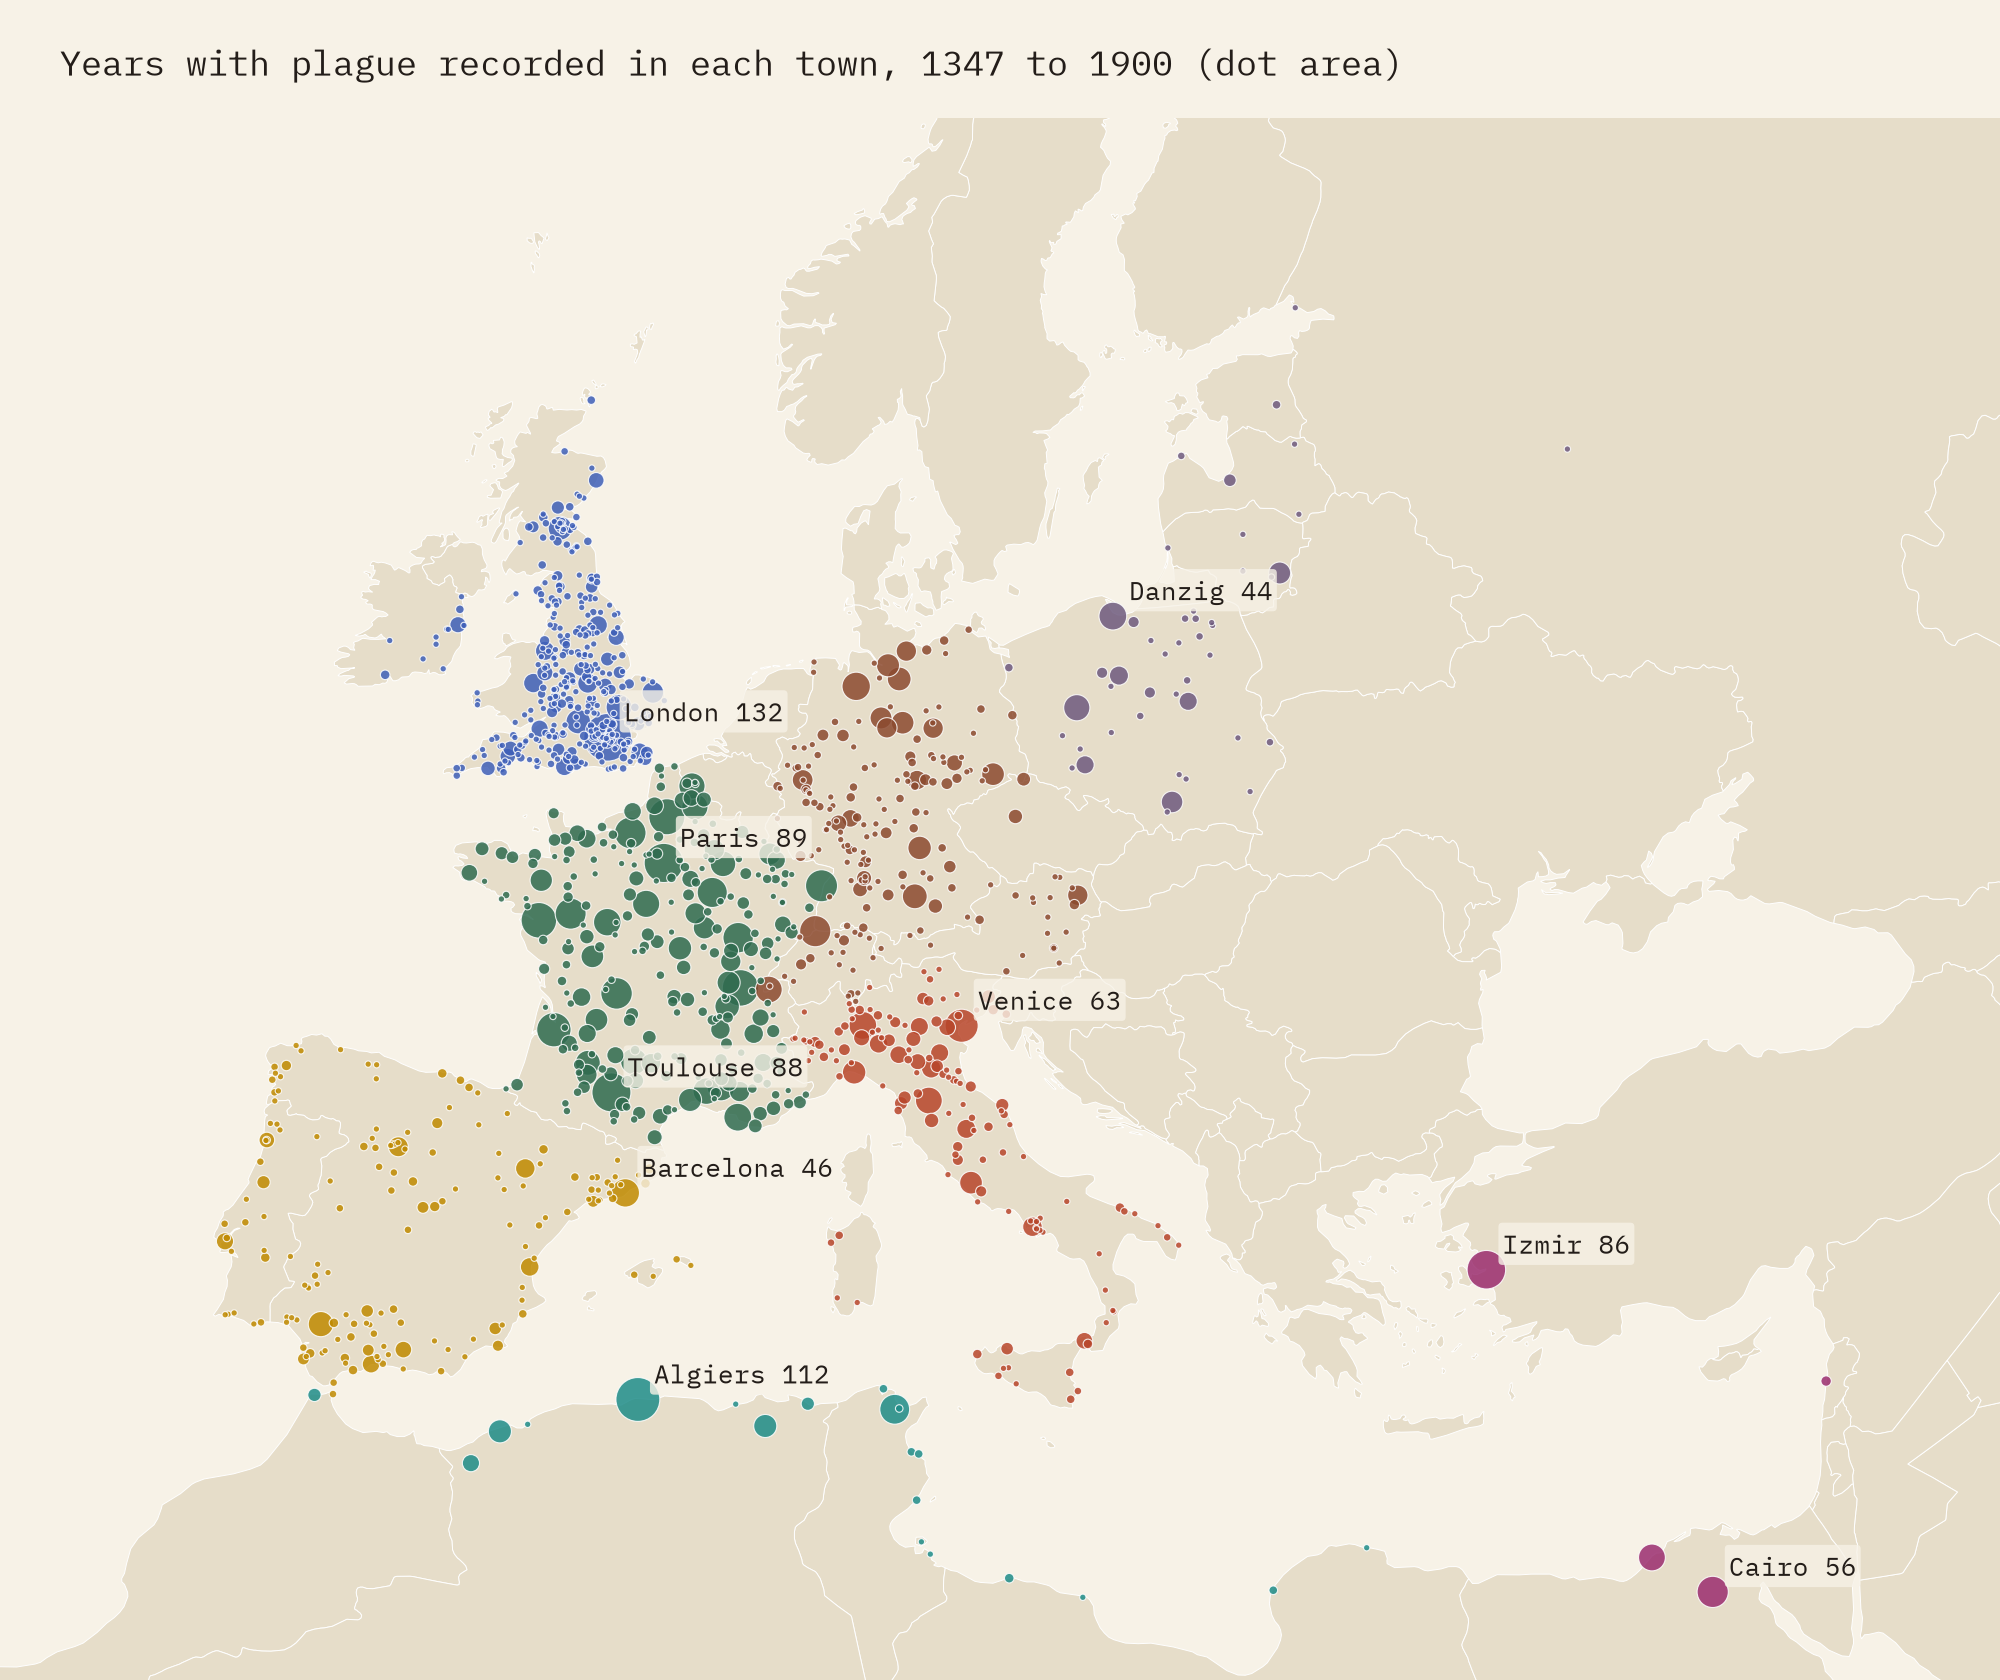
\includegraphics[width=.86\textwidth]{f_often_map.png}
\caption{Years with plague recorded in each town, 1347 to 1900. Dot area is proportional to the number of outbreak years; colour shows the region.}\label{fig:often}\end{figure}

\begin{figure}[tbp]\centering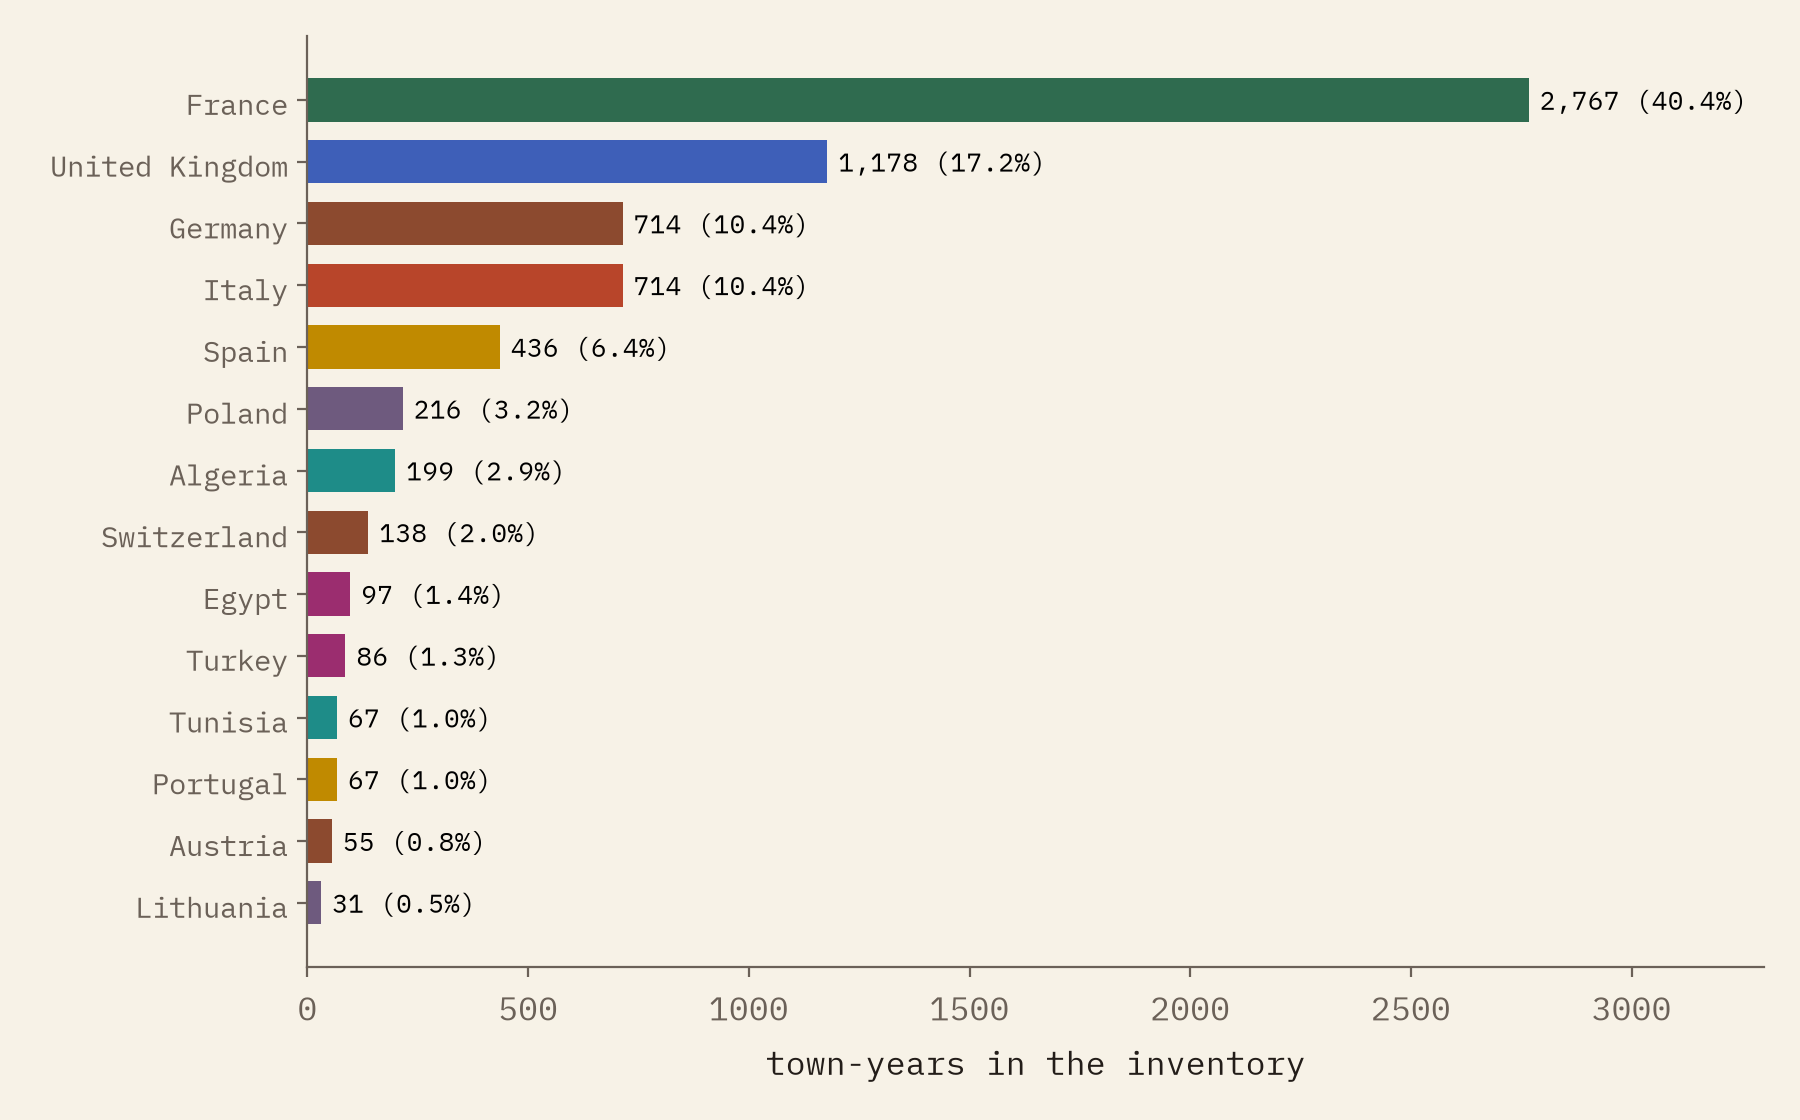
\includegraphics[width=.78\textwidth]{f_coverage.png}
\caption{Town-years by modern country (the 14 countries with most records).}\label{fig:cover}\end{figure}

\subsection{The first wave, 1347 to 1353}
Ten towns have records in 1347, all Mediterranean ports or close to them: Messina, Catania, Syracuse, Trapani, Agrigento and Sciacca in Sicily, Reggio di Calabria, Naples, Genoa and Cagliari. In 1348 plague is recorded in 110 towns, from Alexandria and Cairo to Seville, Bordeaux, London and Bristol, and in Dublin and Drogheda. In 1349 it reaches Paris and the German lands, and in 1350 the Baltic coast, Danzig and Stralsund among them (Figure~\ref{fig:wavemap}). Of the 195 towns first recorded in 1347 to 1353, 189 are in Europe, and 59\% of those were reached by the end of 1348.

\begin{figure}[tbp]\centering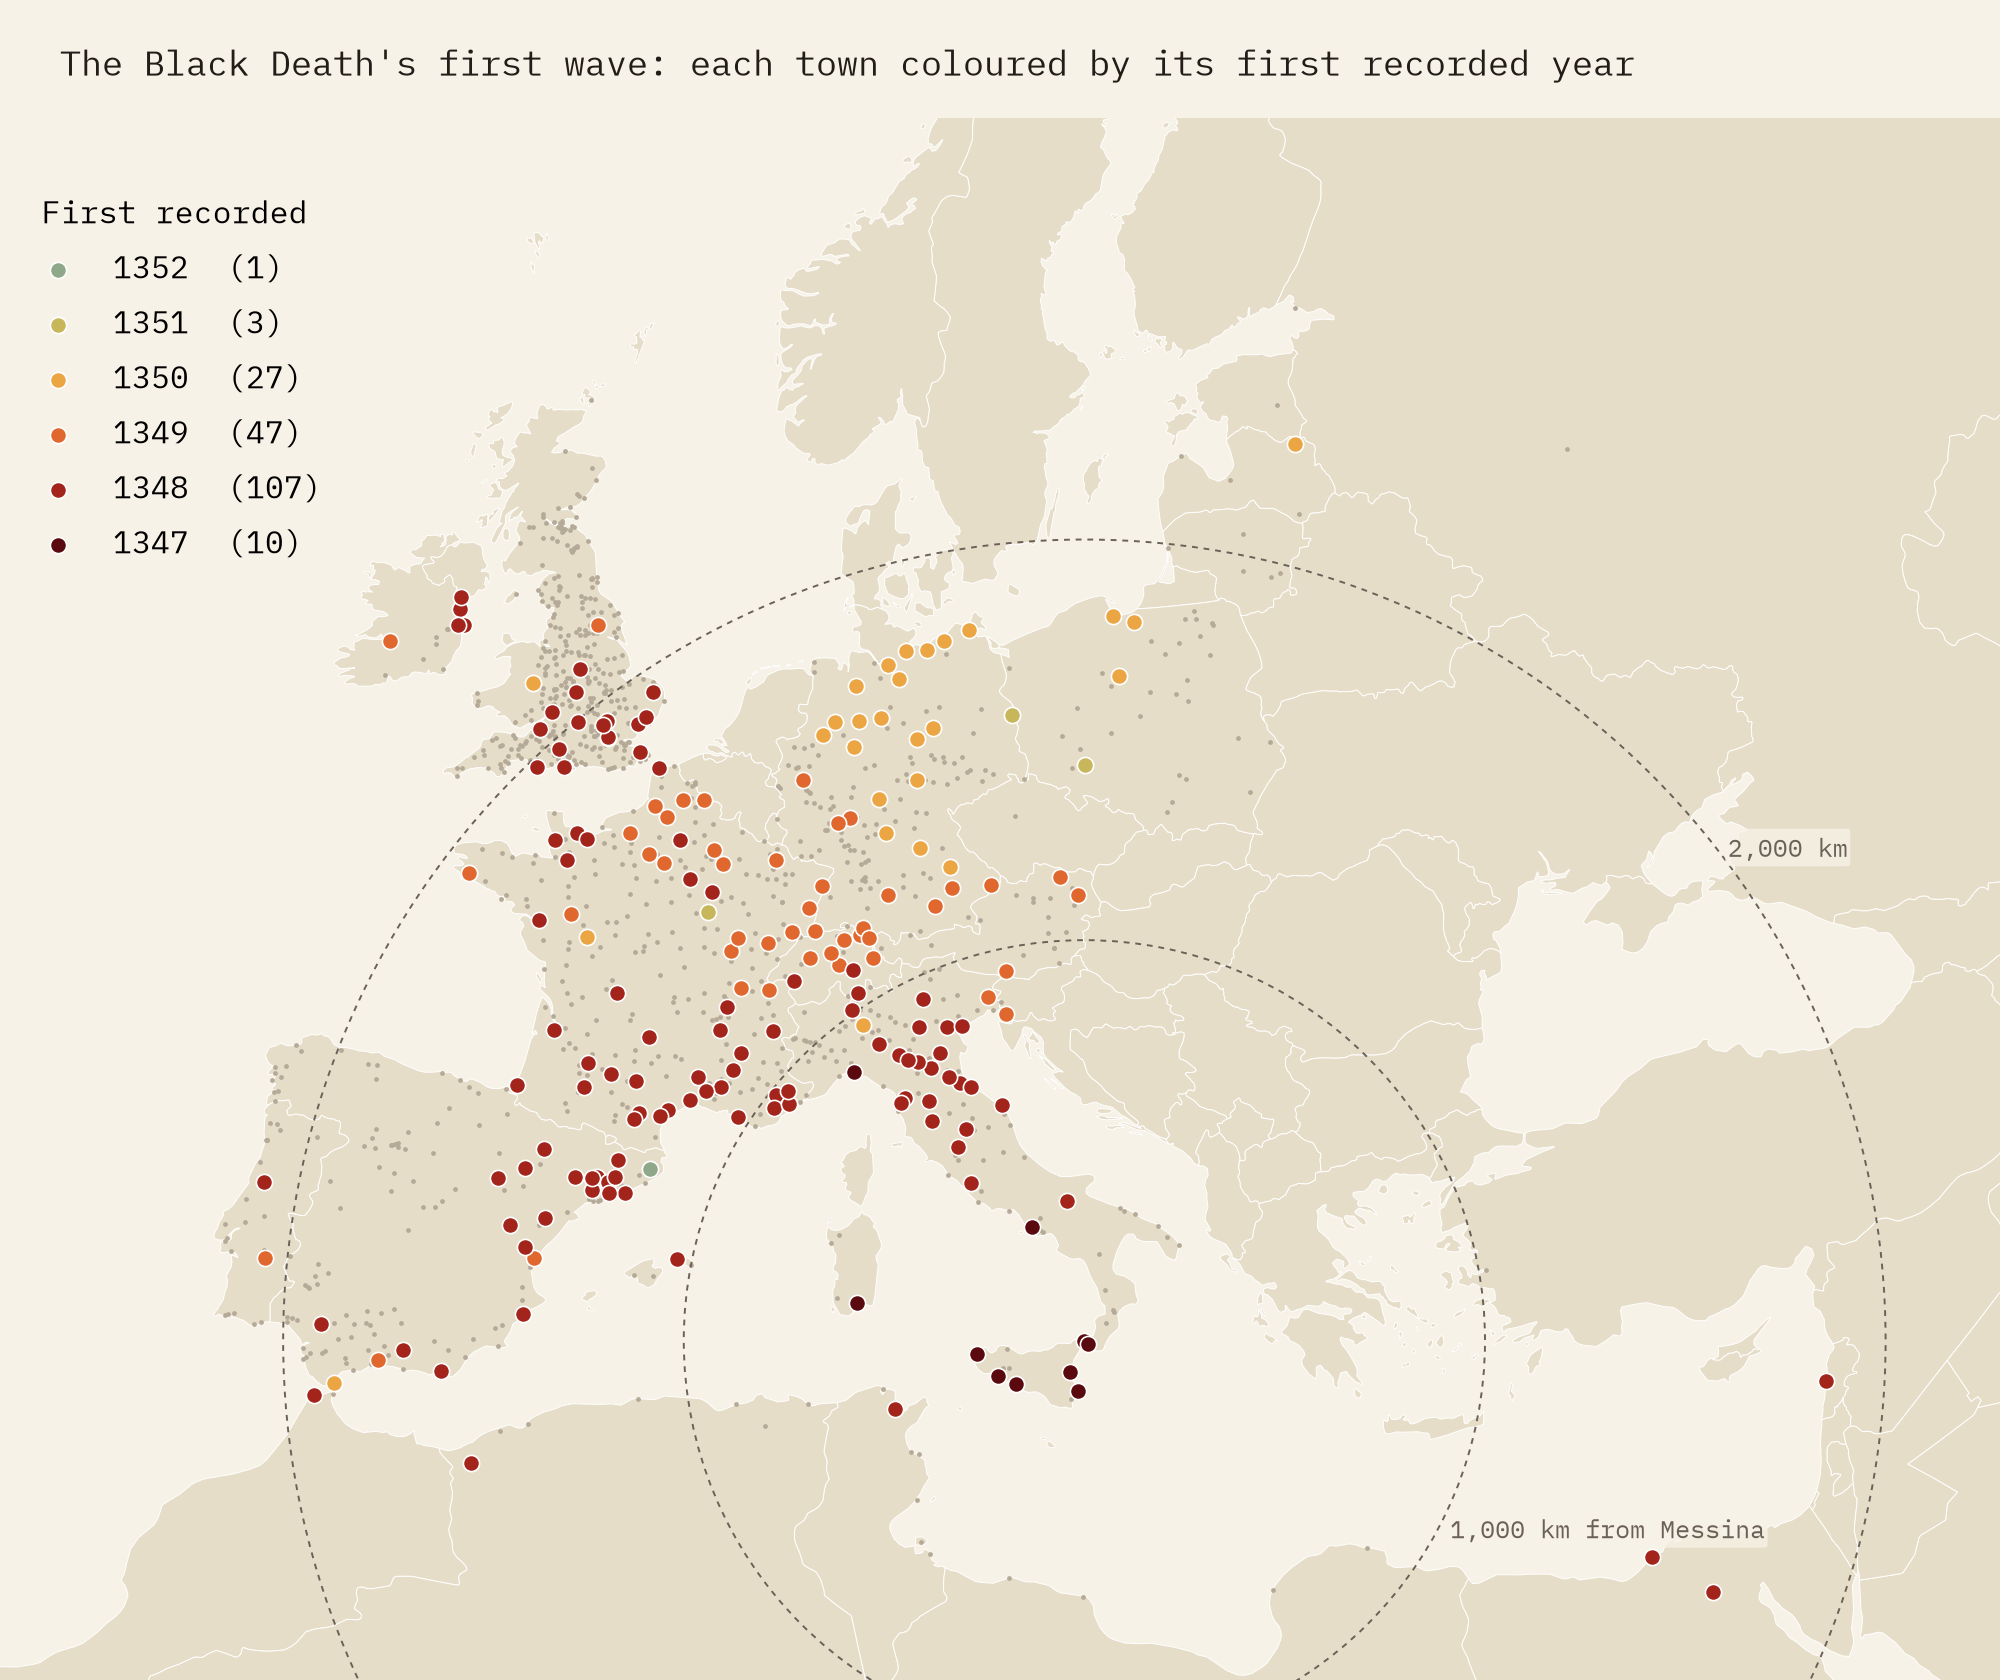
\includegraphics[width=.86\textwidth]{f_wave_map.png}
\caption{The first wave. Each town first recorded in 1347 to 1353 is coloured by that year; grey points are towns first recorded later. Dashed circles are 1,000 and 2,000 km from Messina.}\label{fig:wavemap}\end{figure}

Distance from Messina rises with year, but not smoothly (Figure~\ref{fig:wavedist}). The ten towns of 1347 lie within 885 km of Messina; by the end of 1348, nine in ten of the towns reached lay within 1,974 km and the farthest, Dundalk, was 2,421 km away. Sea routes carried plague to England and Ireland in 1348 while much nearer inland towns were reached in 1349 or 1350. Fitted slopes for the European towns are 176 km a year (Theil-Sen, distance from the nearest 1347 town; bootstrap 95\% interval 112 to 221), 214 km a year (Theil-Sen, distance from Messina) and 202 km a year (least squares, from Messina): about 0.5 to 0.6 km a day. These are averages over sea passages that could cover hundreds of kilometres in weeks and overland movement that was much slower, measured in straight lines and with dates rounded to the year. They describe how the frontier of recorded plague moved outward over four years, not how fast any single journey went.

\begin{figure}[tbp]\centering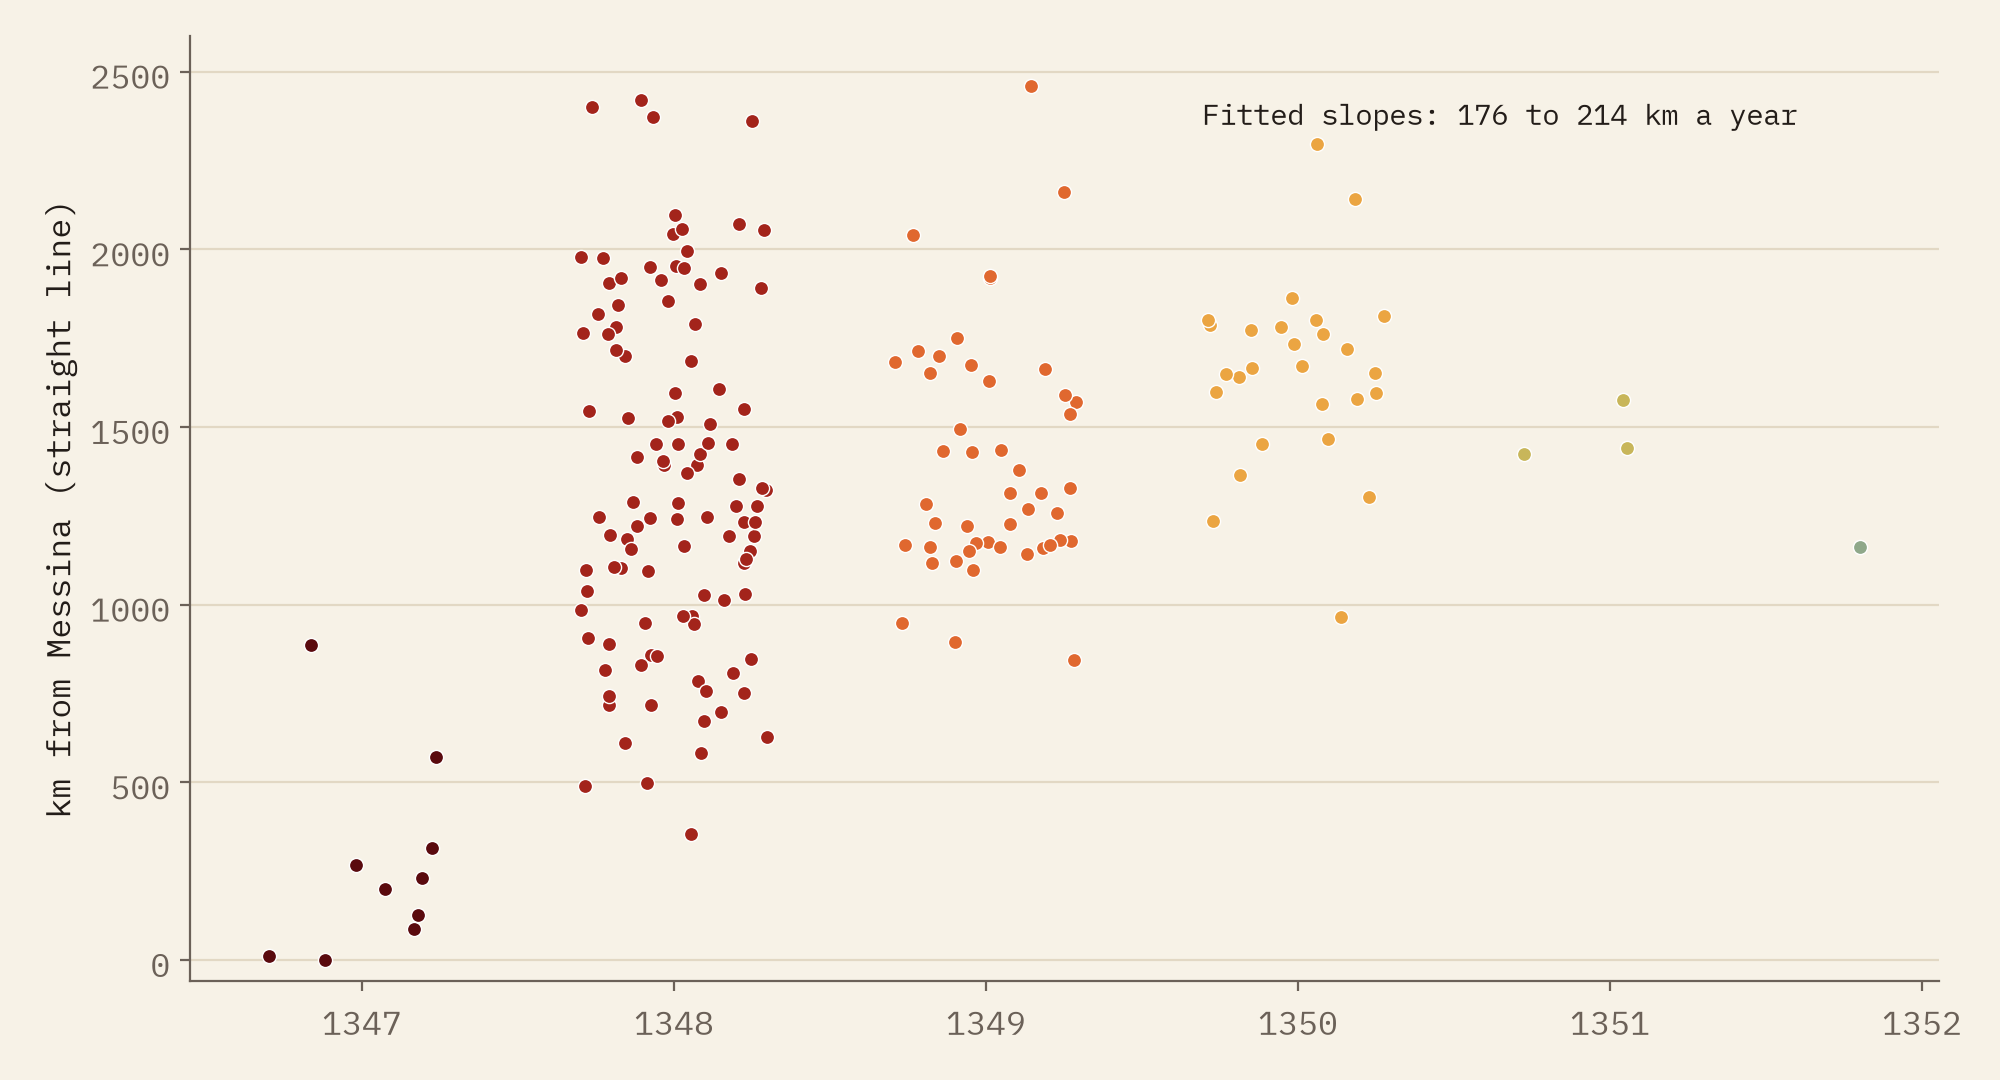
\includegraphics[width=.86\textwidth]{f_wave_distance.png}
\caption{First recorded year and straight-line distance from Messina for the 195 towns of the first wave. Points are spread sideways within each year.}\label{fig:wavedist}\end{figure}

\subsection{Five centuries of outbreaks}
Outbreaks are recorded in almost every decade from the 1340s to the 1660s (Figure~\ref{fig:dec}). The number rises through the fifteenth and sixteenth centuries to a peak in the 1630s, with 570 town-years in 300 towns, mostly in France and northern Italy; the single busiest year is 1630 (119 towns). By century of the outbreak year, the counts are 589 (fourteenth), 1,126 (fifteenth), 2,494 (sixteenth), 2,271 (seventeenth), 286 (eighteenth) and 82 (nineteenth), and 68\% of all town-years fall between 1500 and 1669. Part of this rise is the growth of records: town archives, health boards and printed bills of mortality multiply in the sixteenth and seventeenth centuries, so the earlier centuries are likely to be under-recorded relative to the later. After 1667 the record shrinks to 7.6\% of the total, and from 1720 onwards 86\% of it is in North Africa, Anatolia, the Levant and Egypt.

\begin{figure}[tbp]\centering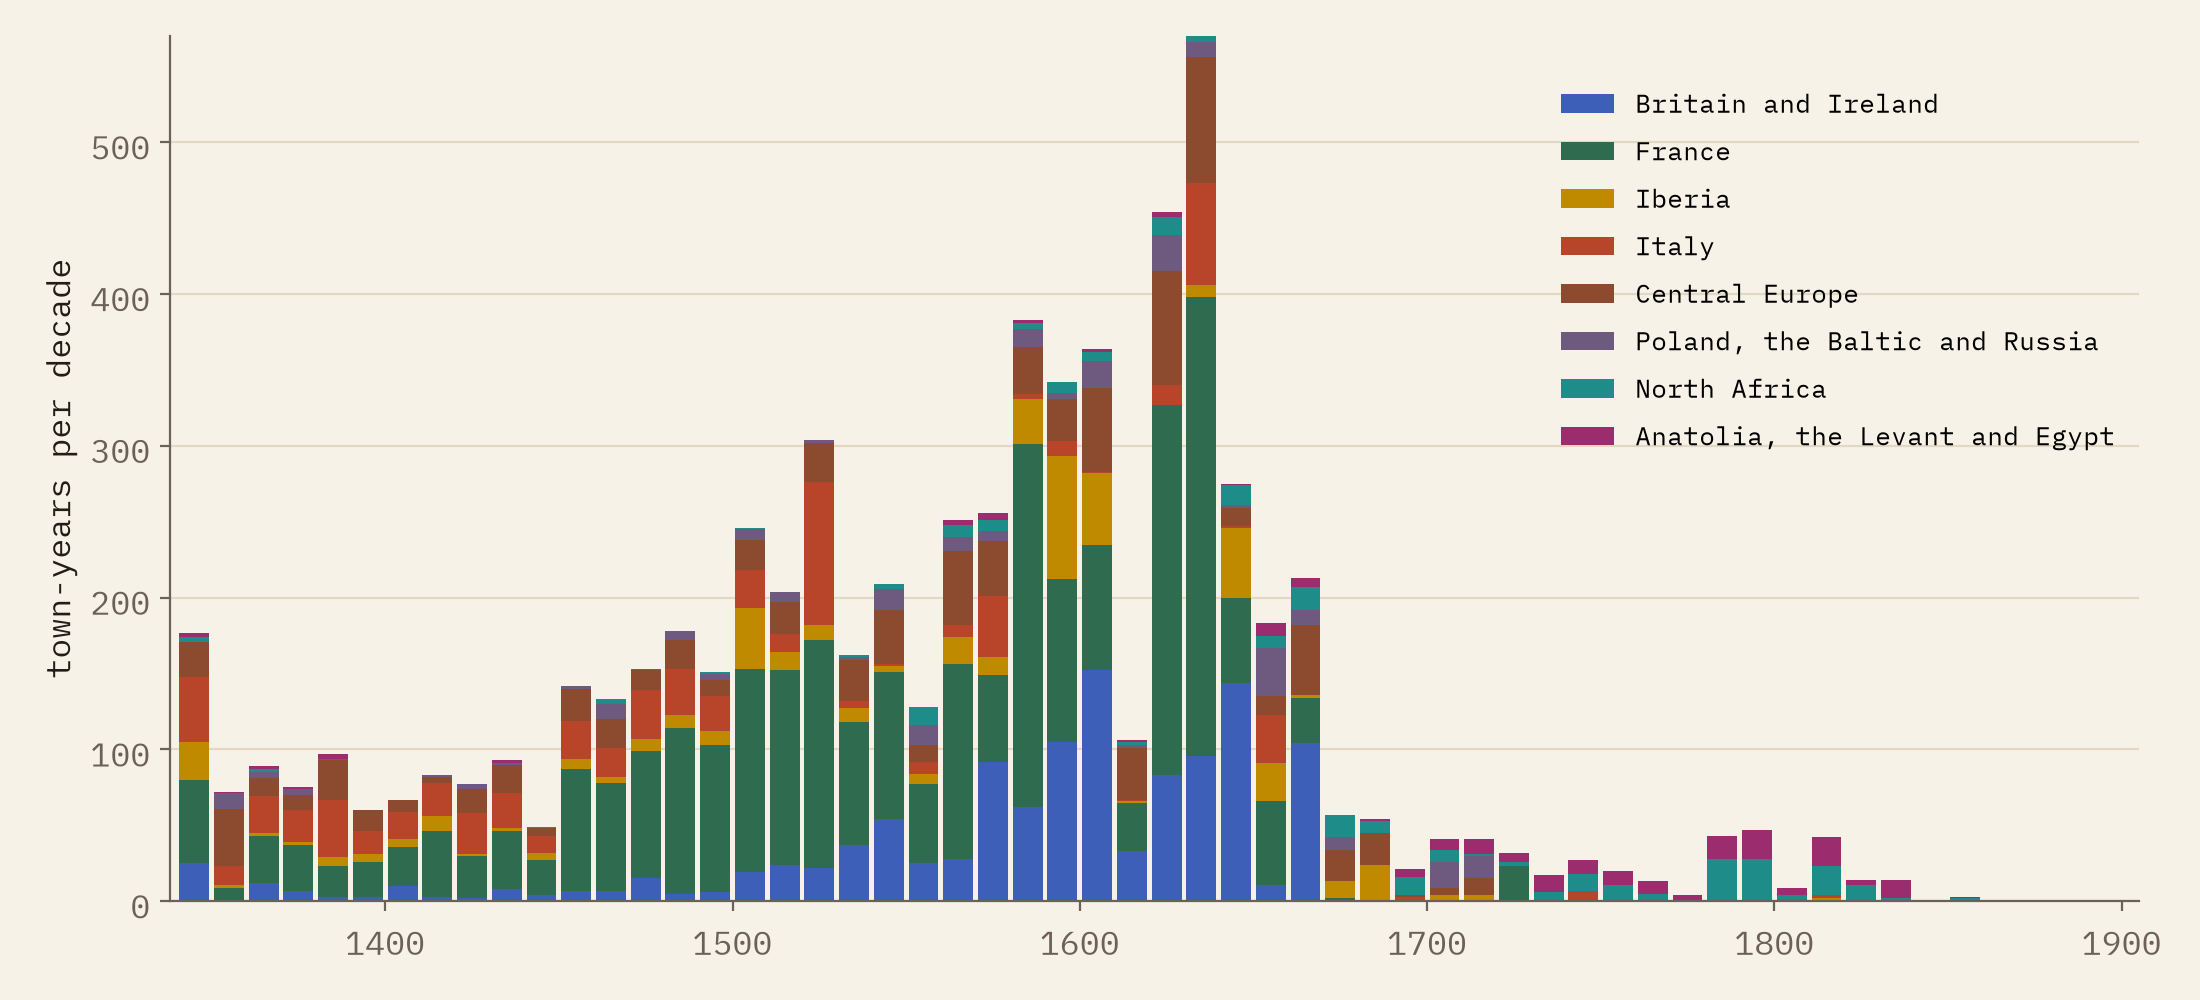
\includegraphics[width=\textwidth]{f_decades.png}
\caption{Town-years with plague recorded per decade, by region.}\label{fig:dec}\end{figure}

\subsection{The towns}
London has the most outbreak years (132, from 1348 to 1667), followed by Algiers (112), Paris (89), Toulouse (88) and Izmir (86) (Figure~\ref{fig:top}, Table~\ref{tab:top}). The twenty towns with most outbreak years hold 21\% of all records. High counts belong to large, connected towns with long runs of records, and often to towns well studied by historians whose work Biraben drew on: London's bills of mortality are an exceptional source, and the long late series for Algiers and Izmir probably owe much to the reports of European consuls and merchants in the Ottoman Mediterranean.

\begin{figure}[tbp]\centering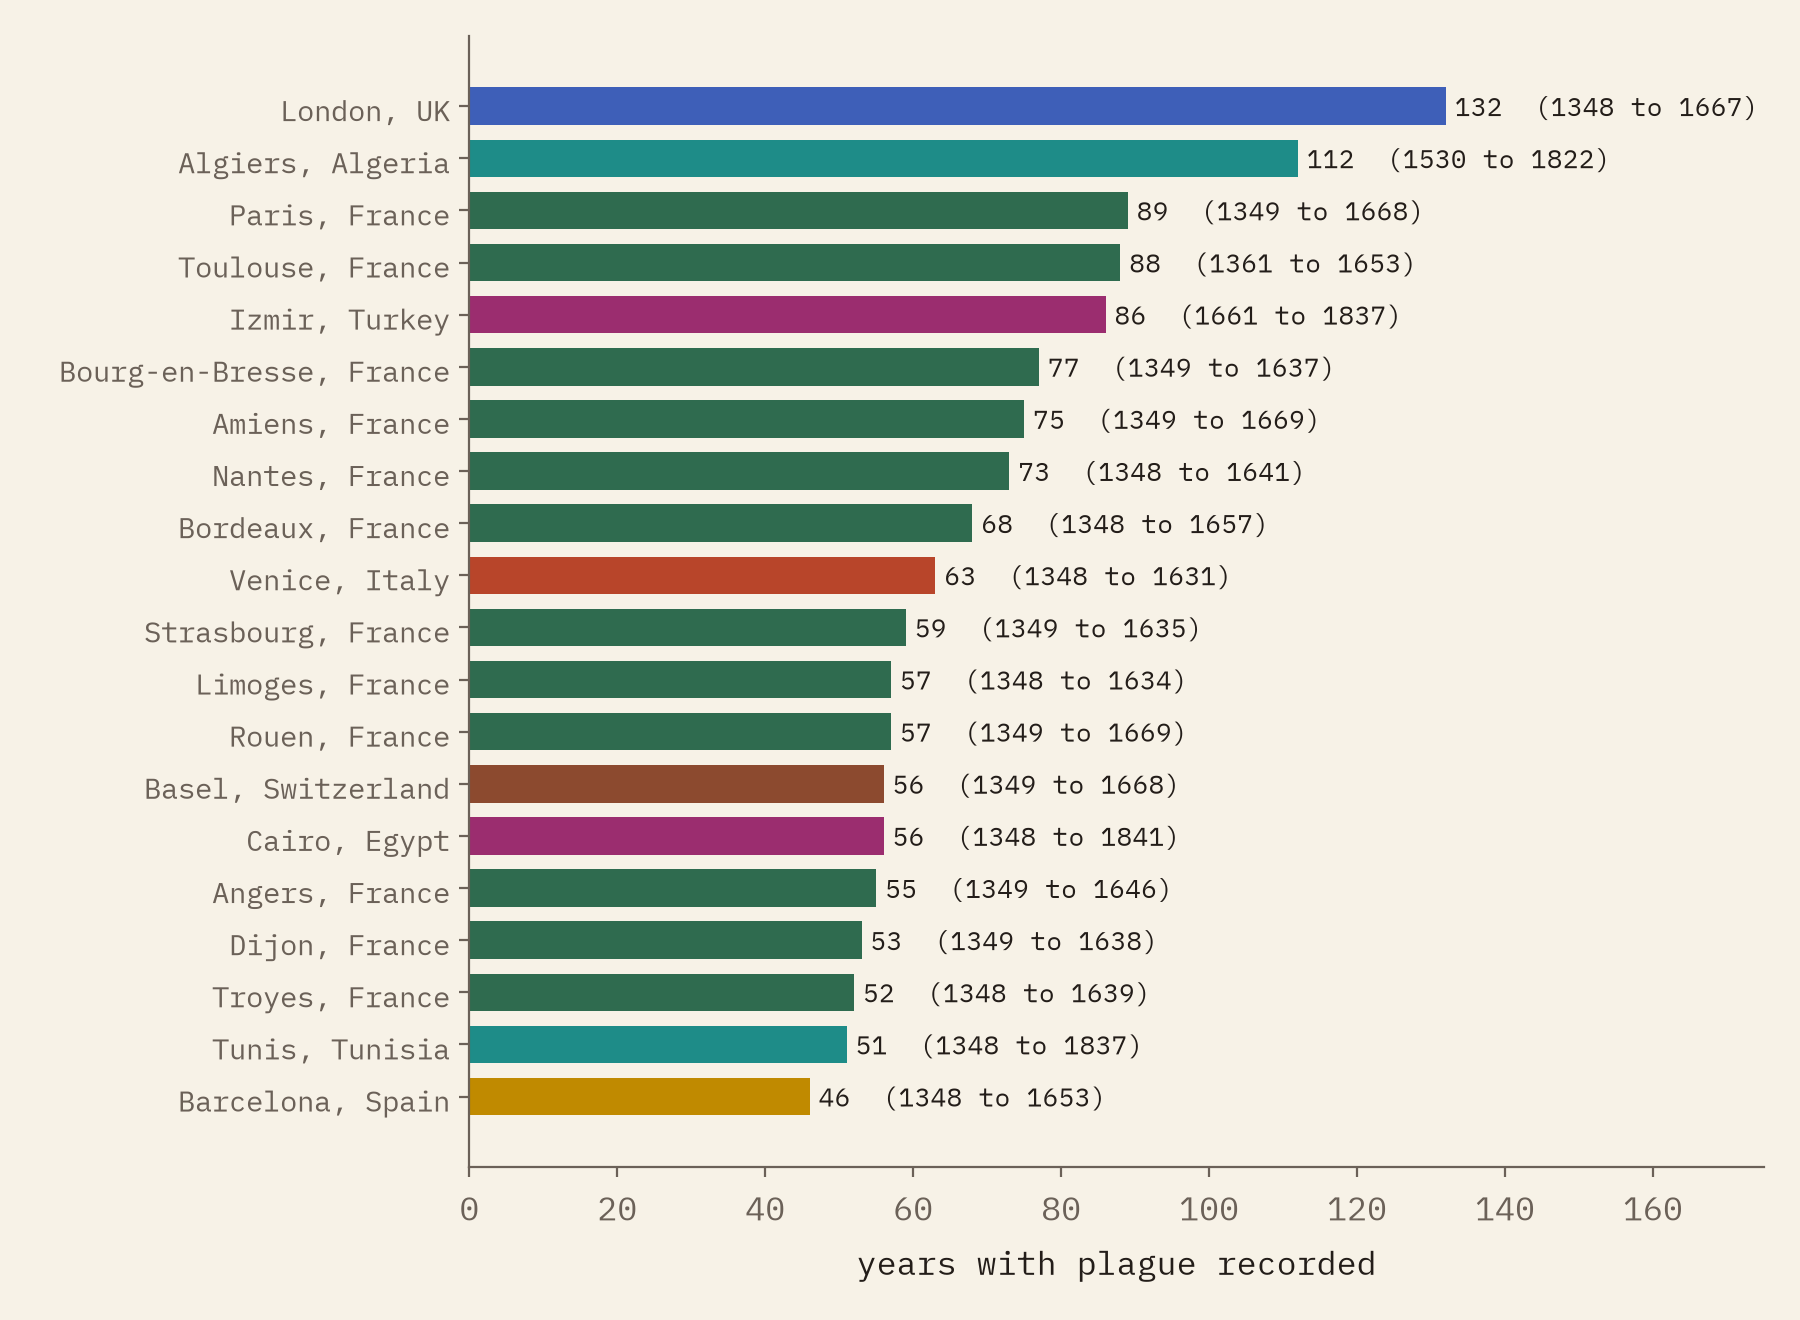
\includegraphics[width=.8\textwidth]{f_top_towns.png}
\caption{The twenty towns with most years with plague recorded, coloured by region.}\label{fig:top}\end{figure}

\begin{table}[tbp]\centering\small\caption{The twenty towns with most outbreak years (names as in the inventory).}\label{tab:top}\begin{tabular}{llrrr}\toprule Town & Country & Years & First & Last\\\midrule
London & United Kingdom & 132 & 1348 & 1667\\
Alger (Algiers) & Algeria & 112 & 1530 & 1822\\
Paris & France & 89 & 1349 & 1668\\
Toulouse & France & 88 & 1361 & 1653\\
Izmir (Izmir (Smyrna)) & Turkey & 86 & 1661 & 1837\\
Bourg-en-Bresse & France & 77 & 1349 & 1637\\
Amiens & France & 75 & 1349 & 1669\\
Nantes & France & 73 & 1348 & 1641\\
Bordeaux & France & 68 & 1348 & 1657\\
Venezia (Venice) & Italy & 63 & 1348 & 1631\\
Strasbourg & France & 59 & 1349 & 1635\\
Limoges & France & 57 & 1348 & 1634\\
Rouen & France & 57 & 1349 & 1669\\
Basel & Switzerland & 56 & 1349 & 1668\\
Kairo (Cairo) & Egypt & 56 & 1348 & 1841\\
Angers & France & 55 & 1349 & 1646\\
Dijon & France & 53 & 1349 & 1638\\
Troyes & France & 52 & 1348 & 1639\\
Tunis & Tunisia & 51 & 1348 & 1837\\
Barcelona & Spain & 46 & 1348 & 1653\\
\bottomrule\end{tabular}\end{table}

\subsection{Recurrence}
Joining consecutive years gives 4,375 episodes, 30\% of them lasting two years or more (mean length 1.6 years), and 3,203 intervals between successive episodes in the same town (Figure~\ref{fig:iv}). The median interval is 13 years, the interquartile range 6 to 31 years, and 56\% of intervals are 15 years or less. Intervals shorten over time: the median is 18.5 years for episodes beginning in the fourteenth century, 13 in the fifteenth, 13 in the sixteenth and 11 in the seventeenth. Among the 114 towns with ten or more episodes the median of each town's median interval is 10.5 years; London's 33 episodes are a median of 7 years apart, with the longest gap 30 years. A return interval of about a decade is consistent with the time needed for a town to refill with people not previously exposed, and with plague's repeated reintroduction by trade \citep{schmid2015}; but a long interval in this record can also be a gap in the sources.

\begin{figure}[tbp]\centering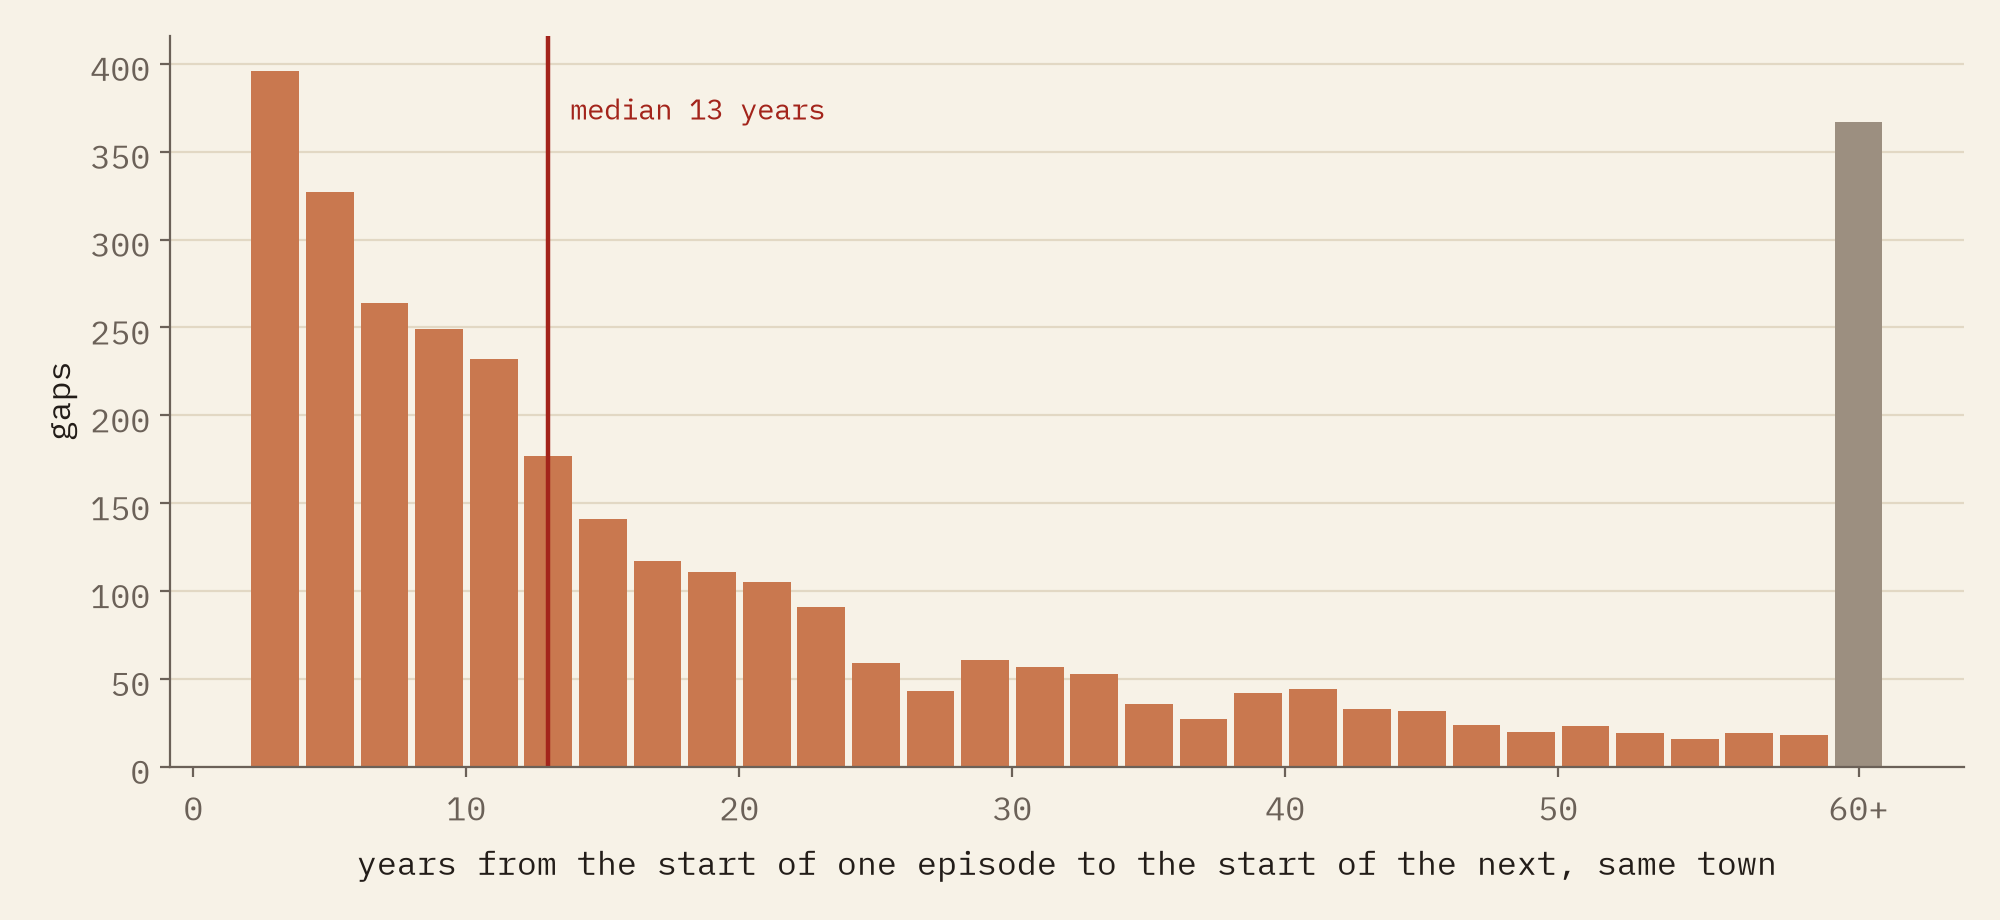
\includegraphics[width=.86\textwidth]{f_intervals.png}
\caption{Intervals from the start of one plague episode to the start of the next in the same town, in two-year bins (last bin: 60 years or more).}\label{fig:iv}\end{figure}

\subsection{When plague left}
Plague's retreat was regional and gradual (Figure~\ref{fig:end}, Table~\ref{tab:regions}). By the last widespread year, it left Italy first (1657, the epidemic of 1656 to 1657 in Naples, Rome and Genoa; on the seventeenth-century Italian epidemics see \citealt{alfani2013}), then Britain and Ireland (1667, the end of the Great Plague of 1665 to 1666, recorded in 57 British towns in 1665), Iberia (1681), Poland and the Baltic (1712), central Europe (1713) and France (1722, the Great Plague of Marseille and Provence, recorded in 10 French towns in 1720 to 1722). In North Africa it remained widespread until 1821 and in Anatolia, the Levant and Egypt until 1834, 167 years after Britain. The last records in each country (Figure~\ref{fig:last}, Table~\ref{tab:countries}) include isolated late outbreaks: Messina in 1743 to 1744, a single year at Marseille in 1786, Noicattaro in 1815 to 1816, Mallorca in 1819, and Porto in 1899 to 1900, an outbreak of the third pandemic rather than the second.

\begin{figure}[tbp]\centering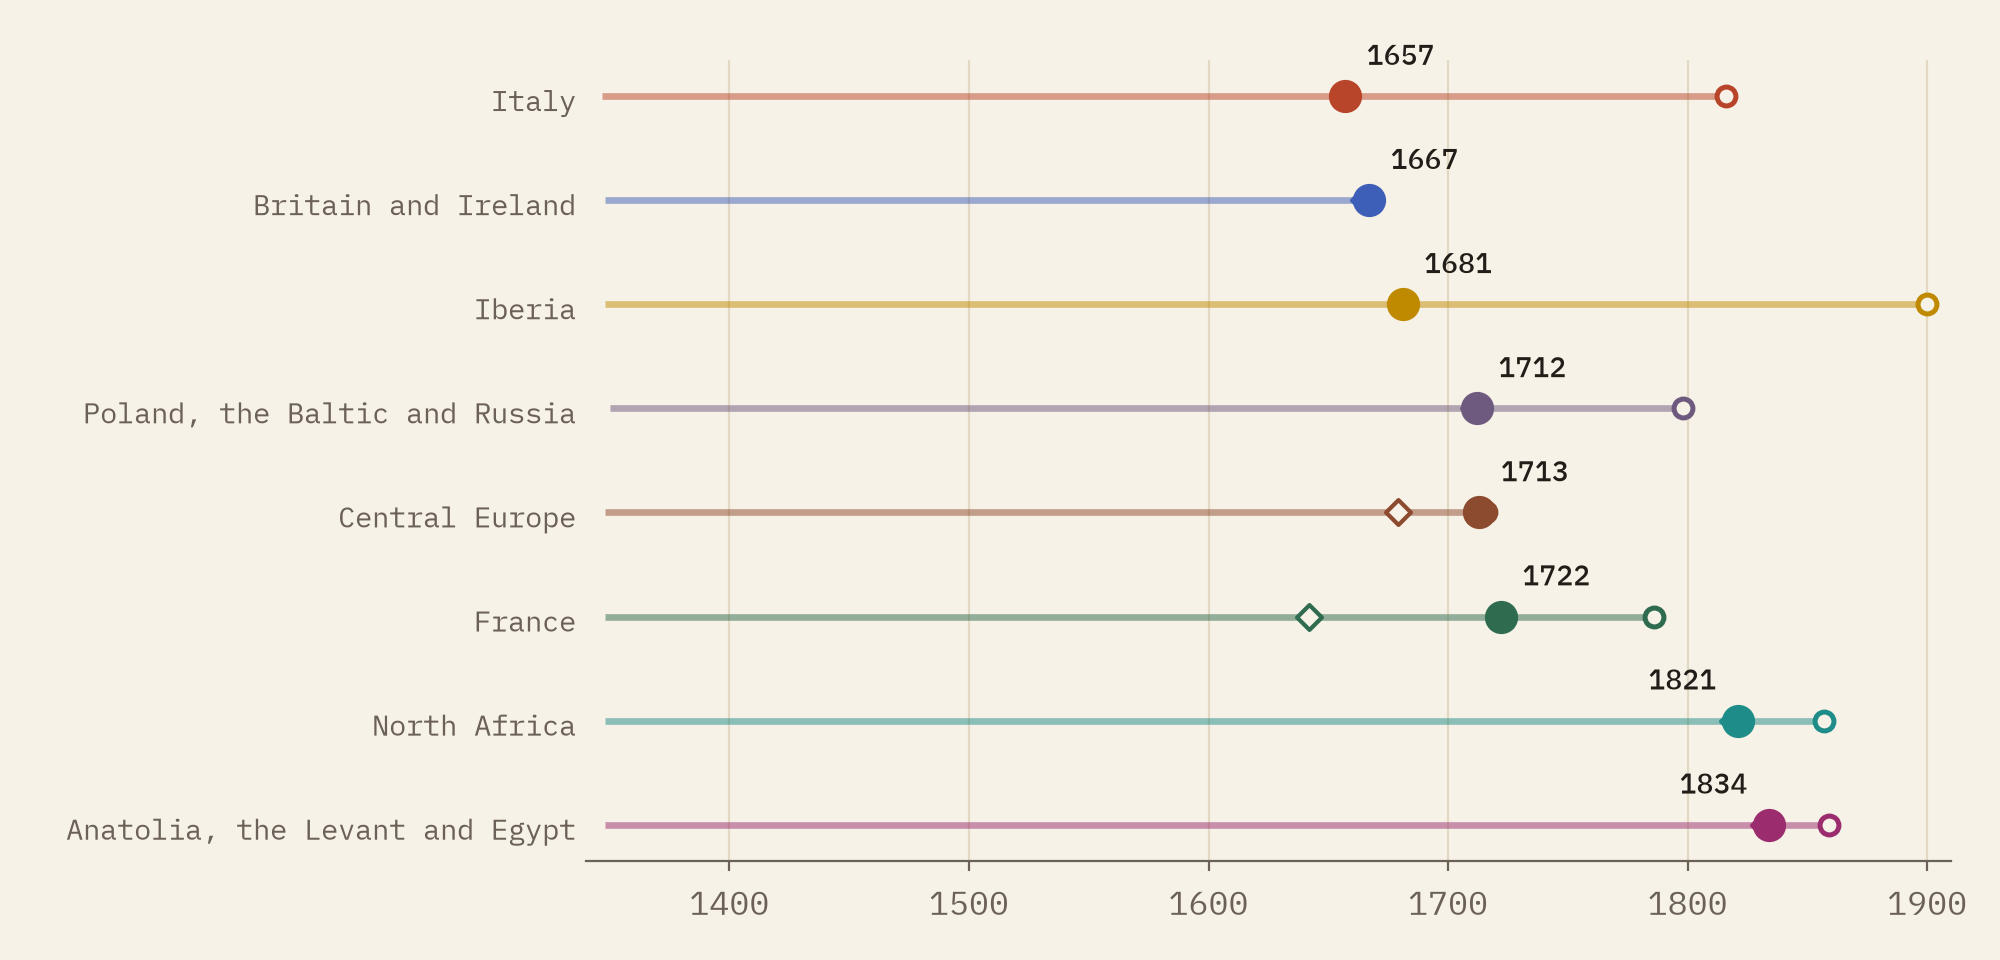
\includegraphics[width=.92\textwidth]{f_end_regions.png}
\caption{When plague left each region. Line: first to last record. Diamond: year by which 95\% of the region's town-years had occurred. Large dot: last year with plague in three or more towns. Ring: last record.}\label{fig:end}\end{figure}

\begin{table}[tbp]\centering\small\caption{Regions: town-years, towns, first record, the year by which 95\% of records had occurred, the last year with plague in three or more towns, and the last record.}\label{tab:regions}\begin{tabular}{lrrrrrr}\toprule Region & Town-years & Towns & First & 95\% & Last 3+ & Last\\\midrule
Italy & 714 & 133 & 1347 & 1656 & 1657 & 1816\\
Britain and Ireland & 1,209 & 374 & 1348 & 1665 & 1667 & 1667\\
Iberia & 503 & 162 & 1348 & 1681 & 1681 & 1900\\
Poland, the Baltic and Russia & 264 & 46 & 1350 & 1711 & 1712 & 1798\\
Central Europe & 919 & 184 & 1348 & 1679 & 1713 & 1716\\
France & 2,767 & 249 & 1348 & 1642 & 1722 & 1786\\
North Africa & 284 & 20 & 1348 & 1819 & 1821 & 1857\\
Anatolia, the Levant and Egypt & 188 & 4 & 1348 & 1832 & 1834 & 1859\\
\bottomrule\end{tabular}\end{table}

\begin{figure}[tbp]\centering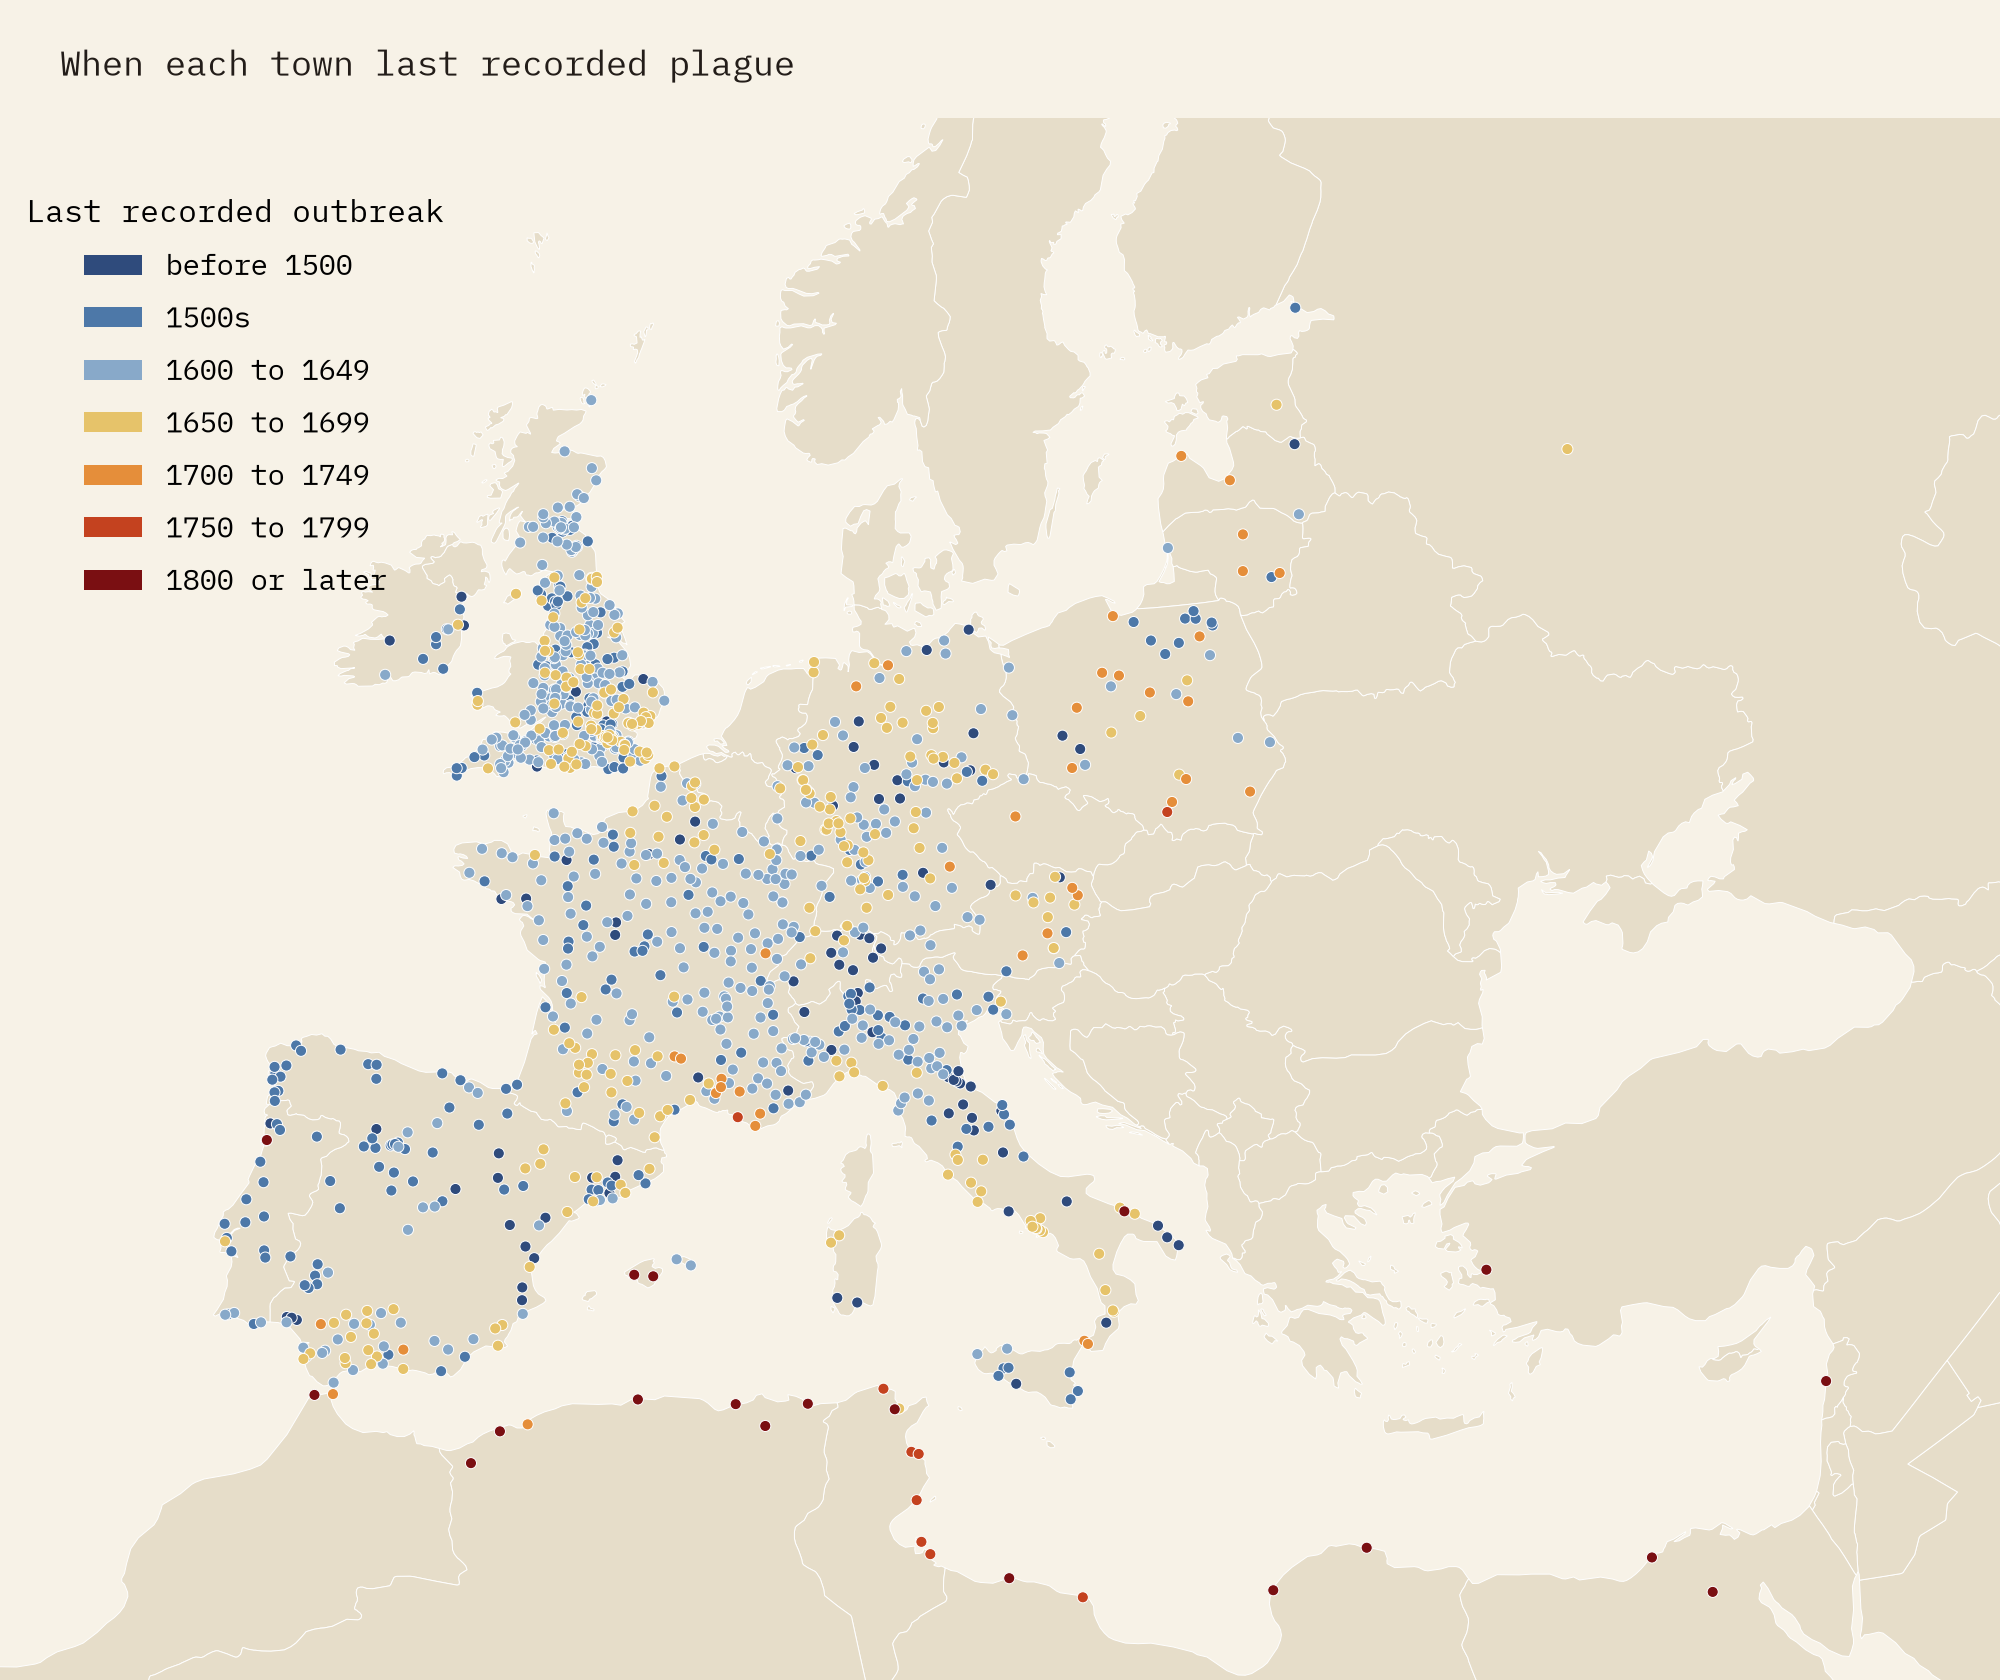
\includegraphics[width=.86\textwidth]{f_last_map.png}
\caption{The last recorded outbreak in each town.}\label{fig:last}\end{figure}

\begin{table}[tbp]\centering\small\caption{Modern countries, sorted by last record.}\label{tab:countries}\setlength{\tabcolsep}{4pt}\begin{tabular}{lrrrrrl}\toprule Country & Town-years & Towns & First & Last 3+ & Last & Last record at\\\midrule
Portugal & 67 & 23 & 1348 & 1599 & 1900 & Porto\\
Lebanon & 5 & 1 & 1348 &  & 1859 & Beirut\\
Libya & 9 & 4 & 1589 &  & 1857 & Benghazi\\
Egypt & 97 & 2 & 1348 &  & 1841 & Cairo\\
Turkey & 86 & 1 & 1661 &  & 1837 & Izmir (Smyrna)\\
Tunisia & 67 & 8 & 1348 & 1785 & 1837 & Tunis\\
Algeria & 199 & 7 & 1348 & 1821 & 1835 & Constantine\\
Morocco & 9 & 1 & 1348 &  & 1819 & Tangier\\
Spain & 436 & 139 & 1348 & 1681 & 1819 & Manacor, Palma\\
Italy & 714 & 133 & 1347 & 1657 & 1816 & Noicattaro\\
Poland & 216 & 34 & 1350 & 1711 & 1798 & Lanckorona\\
France & 2,767 & 249 & 1348 & 1722 & 1786 & Marseille\\
Austria & 55 & 22 & 1349 & 1679 & 1716 & Bruck an der Mur\\
Germany & 714 & 136 & 1349 & 1682 & 1713 & Bremen, Hamburg\\
Czech Republic & 11 & 1 & 1380 &  & 1713 & Prague\\
Latvia & 12 & 4 & 1350 &  & 1712 & Mazirbe\\
Lithuania & 31 & 5 & 1419 & 1711 & 1712 & Vilnius\\
Slovenia & 1 & 1 & 1682 &  & 1682 & Gorizia\\
Switzerland & 138 & 24 & 1348 & 1666 & 1670 & Bern\\
Russia & 2 & 2 & 1564 &  & 1667 & Podol'sk\\
United Kingdom & 1,178 & 361 & 1348 & 1667 & 1667 & Burlington, London, Norwich...\\
Isle of Man & 1 & 1 & 1666 &  & 1666 & Ramsey\\
Estonia & 3 & 1 & 1656 &  & 1658 & Tartu\\
Ireland & 30 & 12 & 1348 & 1575 & 1650 & Dublin\\
\bottomrule\end{tabular}\end{table}

\section{Discussion}
The digitised inventory reproduces the broad shape of the second pandemic as historians describe it: a first wave carried along the sea lanes of the Mediterranean and Atlantic and then overland, recurrent epidemics for three centuries, a peak in the early seventeenth century, and a retreat from western Europe in the late seventeenth and early eighteenth centuries that left plague in the Ottoman Mediterranean for another hundred years. The order of retreat in this record, Italy and Britain before France, central Europe and the Baltic, and all of them a century before North Africa and the Levant, is clear even allowing for single stray records.

Two features of the record deserve emphasis. First, the eastern side of the map is thin. There are no records for the Low Countries, Scandinavia, Hungary or the Balkans beyond Slovenia, only 2 for Russia, none for Moscow's epidemic of 1771, and none for Constantinople, one of the most plague-stricken cities of the period. Second, the western side is dense in proportion to archives and scholarship, not only to plague. France's share reflects Biraben's own focus. The record is best read as a map of where plague was documented, and comparisons between regions as comparisons between documentary traditions as much as between epidemics \citep{roosen2018}.

\section{Limitations}
First, the data record presence, not intensity: a year with a handful of cases and a year that killed half a town count the same. Second, coverage follows surviving documents and Biraben's sources, so absence of records is not absence of plague, especially in eastern Europe and the Ottoman world. Third, some years in the inventory are approximate, and an outbreak spanning two calendar years may appear in one or both. Fourth, diagnoses of `plague' in older sources may include other epidemic diseases. Fifth, places were geocoded automatically; I corrected five clear errors, but others surely remain, and some names are ambiguous. Sixth, the first-wave speeds rest on annual dates and straight-line distances and should be read as coarse summaries. Finally, region and country assignments use modern borders.

\section{Conclusion}
Digitised and lightly repaired, Biraben's inventory gives a vivid year-by-year picture of five centuries of plague in 1,172 towns: the first wave, the repeated returns about once a decade, and a regional retreat that ended in western Europe by the 1720s and in the Ottoman Mediterranean only in the nineteenth century. It is also a picture of where people wrote plague down. The interactive atlas lets readers explore both.

\section*{Data and code availability}
The interactive atlas is at \url{https://maps.tristanhotham.com/plague-map/}. Data and code are at \url{https://github.com/Tristan-Hotham/plague-map} and archived with this paper at \url{https://doi.org/10.5281/zenodo.23844513}. The derived tables are a derived database of the EnviDat dataset and are released under the Open Database Licence 1.0; the text and figures are released under CC BY 4.0 and the code under the MIT licence.

\section*{AI statement}
I wrote the text, with drafting and editing assistance from Claude (Anthropic), which also helped prepare the analysis code. I reviewed and checked all text and results.

\begin{thebibliography}{9}
\bibitem[Alfani(2013)]{alfani2013} Alfani, G. (2013) Plague in seventeenth-century Europe and the decline of Italy: an epidemiological hypothesis. \emph{European Review of Economic History}, 17(4), 408 to 430.
\bibitem[Benedictow(2004)]{benedictow2004} Benedictow, O.J. (2004) \emph{The Black Death 1346 to 1353: the complete history}. Woodbridge: Boydell Press.
\bibitem[Biraben(1975)]{biraben1975} Biraben, J.-N. (1975 to 1976) \emph{Les hommes et la peste en France et dans les pays europ\'eens et m\'editerran\'eens}. 2 vols. Paris and The Hague: Mouton.
\bibitem[B\"untgen et~al.(2012)]{buntgen2012} B\"untgen, U., Ginzler, C., Esper, J., Tegel, W. and McMichael, A.J. (2012) Digitizing historical plague. \emph{Clinical Infectious Diseases}, 55(11), 1586 to 1588.
\bibitem[EnviDat(2012)]{envidat} B\"untgen, U., Ginzler, C., Esper, J., Tegel, W. and McMichael, A.J. Historical plague outbreaks in Europe. EnviDat. doi:10.16904/envidat.181. Open Database Licence 1.0.
\bibitem[G\'omez and Verd\'u(2017)]{gomez2017} G\'omez, J.M. and Verd\'u, M. (2017) Network theory may explain the vulnerability of medieval human settlements to the Black Death pandemic. \emph{Scientific Reports}, 7, 43467.
\bibitem[Natural Earth(2026)]{naturalearth} Natural Earth (2026) Admin 0 countries (1:10m and 1:50m) and populated places. Public domain. \url{https://www.naturalearthdata.com/}
\bibitem[Roosen and Curtis(2018)]{roosen2018} Roosen, J. and Curtis, D.R. (2018) Dangers of noncritical use of historical plague data. \emph{Emerging Infectious Diseases}, 24(1), 103 to 110.
\bibitem[Schmid et~al.(2015)]{schmid2015} Schmid, B.V., B\"untgen, U., Easterday, W.R., Ginzler, C., Walløe, L., Bramanti, B. and Stenseth, N.C. (2015) Climate-driven introduction of the Black Death and successive plague reintroductions into Europe. \emph{Proceedings of the National Academy of Sciences}, 112(10), 3020 to 3025.
\end{thebibliography}
\end{document}
